\chapter{Classificazione dei Design Pattern per Smart-Contract}
I design pattern adottati nello sviluppo di smart-contract possono essere classificati in diversi tipi\cite[alcuni tipi]{9089272}\cite{9050163}, ognuno dei quali caratterizza un aspetto specifico della lifecycle del contratto:

\begin{itemize}
	\item \textit{Authorization}: relativi alla gestione dell'accesso alle funzionalità del contratto;
	\item \textit{Behavioral}: relativi a meccanismi di supporto per il corretto svolgimento delle funzionalità del contratto;
	\item \textit{Gas Economic}: relativi a meccanismi per ridurre il consumo di \textit{gas} durante l'esecuzione delle funzionalità del contratto;
	\item \textit{Lifecycle}: relativi alla a meccanismi per la creazione e la distruzione del contratto;
	\item \textit{Maintenance}: relativi a meccanismi di supporto per la manutenzione del contratto;
	\item \textit{Security}: relativi a meccanismi per la mitigazione di vulnerabilità di sicurezza note;
\end{itemize}

\section{Authorization Design Pattern}
La blockchain di Ethereum non implementa meccanismi di autenticazione o di ruoli/permessi per consentire l'accesso alle funzionalità di un contratto solo nel caso in cui vengano soddisfatte determinate condizioni. Per la natura della blockchain, ogni funzione definita con visibilità pubblica può essere invocata da qualsiasi utente.\par
Gli \textit{Authorization Design Pattern} offrono meccanismi atti a limitare l'esecuzione delle funzionalità di un contratto. Si individuano i seguenti design pattern: \textit{Ownership} e \textit{Access Restriction}.
\subsection{Ownership Pattern}
L’\textit{Ownership} pattern offre un meccanismo per riservare al proprietario di uno smart-contract l’esecuzione di funzionalità critiche, a cui l’utente finale non deve avere accesso.\par
Opzionalmente possono essere implementati anche meccanismi di supporto per eseguire l’operazione di trasferimento del titolo di proprietario.
\begin{table}[H]\label{Ownership_table}
	\caption{Specifiche dell'Ownership Pattern}
	\centering
	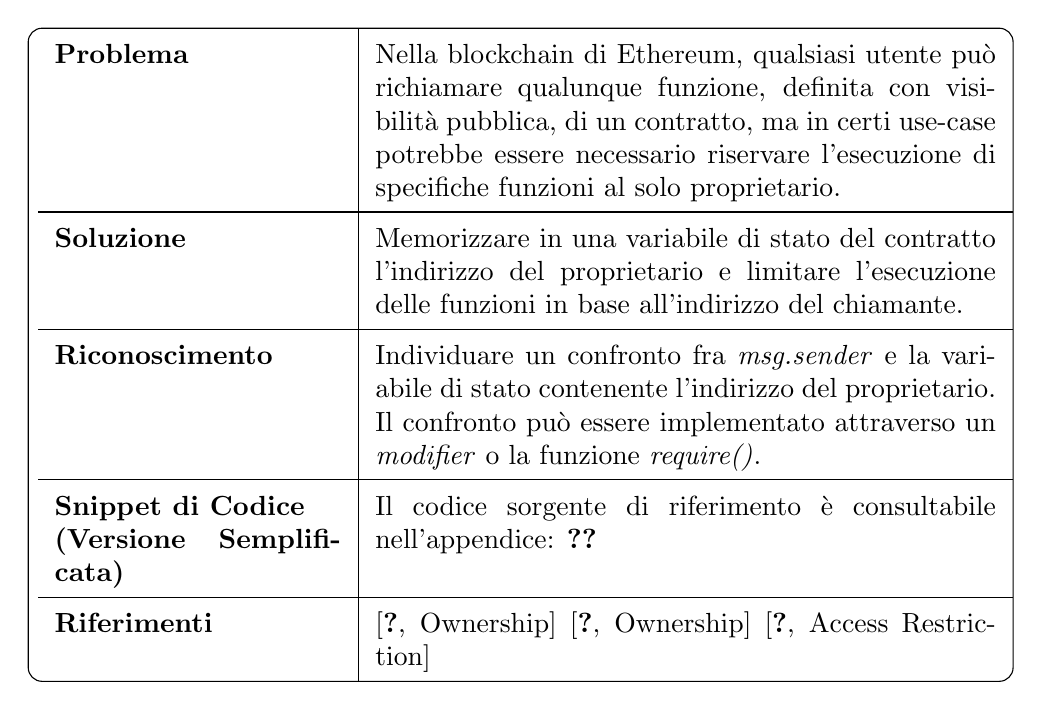
\begin{tikzpicture}
		\node (table) [inner sep=0pt] {
			\def\arraystretch{1.5}
			\begin{tabular}{p{0.30\linewidth} | p{0.65\linewidth}}
				\textbf{Problema} & {Nella blockchain di Ethereum, qualsiasi utente può richiamare qualunque funzione, definita con visibilità pubblica, di un contratto, ma in certi use-case potrebbe essere necessario riservare l’esecuzione di specifiche funzioni al solo proprietario.} \\ \hline
				\textbf{Soluzione} & {Memorizzare in una variabile di stato del contratto l'indirizzo del proprietario e limitare l'esecuzione delle funzioni in base all'indirizzo del chiamante.} \\ \hline
				\textbf{Riconoscimento} & {Individuare un confronto fra \textit{msg.sender} e la variabile di stato contenente l’indirizzo del proprietario.\par Il confronto può essere implementato attraverso un \textit{modifier} o la funzione \textit\mbox{\textit{require()}}.} \\ \hline
				\textbf{Snippet di Codice\newline(Versione Semplificata)} & Il codice sorgente di riferimento è consultabile nell'appendice: \ref{appendix:ownership}  \\ \hline
				\textbf{Riferimenti} & \cite[Ownership]{maxwoe} \cite[Ownership]{cjgdev} \cite[Access Restriction]{fravoll} \\
			\end{tabular}
		};
		\draw [rounded corners=.5em] (table.north west) rectangle (table.south east);
	\end{tikzpicture}
\end{table}
\newpage
\subsection{Access Restriction Pattern}
L’\textit{Ownership} pattern offre un meccanismo per riservare al proprietario di uno smart-contract l’esecuzione di funzionalità critiche, a cui l’utente finale non deve avere accesso.\par
Opzionalmente possono essere implementati anche meccanismi di supporto per eseguire l’operazione di trasferimento del titolo di proprietario.
\begin{table}[H]\label{Access_Restriction_table}
	\caption{Specifiche dell'Ownership Pattern}
	\centering
	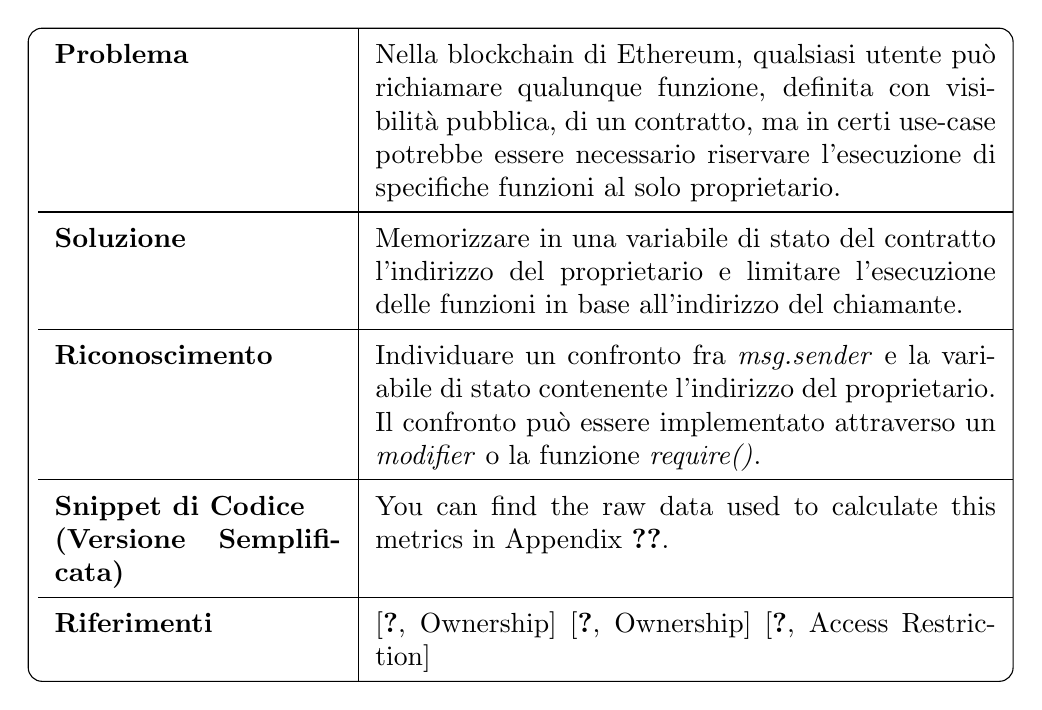
\begin{tikzpicture}
		\node (table) [inner sep=0pt] {
			\def\arraystretch{1.5}
			\begin{tabular}{p{0.30\linewidth} | p{0.65\linewidth}}
				\textbf{Problema} & {Nella blockchain di Ethereum, qualsiasi utente può richiamare qualunque funzione, definita con visibilità pubblica, di un contratto, ma in certi use-case potrebbe essere necessario riservare l’esecuzione di specifiche funzioni al solo proprietario.} \\ \hline
				\textbf{Soluzione} & {Memorizzare in una variabile di stato del contratto l'indirizzo del proprietario e limitare l'esecuzione delle funzioni in base all'indirizzo del chiamante.} \\ \hline
				\textbf{Riconoscimento} & {Individuare un confronto fra \textit{msg.sender} e la variabile di stato contenente l’indirizzo del proprietario.\par Il confronto può essere implementato attraverso un \textit{modifier} o la funzione \textit\mbox{\textit{require()}}.} \\ \hline
				\textbf{Snippet di Codice\newline(Versione Semplificata)} & 
				You can find the raw data used to calculate this metrics in Appendix \ref{appendix:ownership}.\\ \hline
				\textbf{Riferimenti} & \cite[Ownership]{maxwoe} \cite[Ownership]{cjgdev} \cite[Access Restriction]{fravoll} \\
			\end{tabular}
		};
		\draw [rounded corners=.5em] (table.north west) rectangle (table.south east);
	\end{tikzpicture}
\end{table}